\section{Adapter Ablation}
\label{supp:adapter}
The static adapter improves on the official reference in the evaluated ETTh1 condition, while global-statistics FiLM does not improve over matched static capacity.
\begin{table}[ht]\centering\caption{Static and missingness-aware adapter comparison on ETTh1 random-0.3.}\label{tab:supp-adapter}\scriptsize\begin{tabular}{@{}lrrrrrr@{}}
\toprule
Variant & Trainable & Overhead & Best epoch & Val. MSE & Test MSE & Test MAE \\
\midrule
Official & 0 & 0.00\% & NA & NA & 0.425394 & 0.450336 \\
Static adapter & 33,600 & 2.96\% & 1 & 0.678666 & 0.361377 & 0.390458 \\
Missingness-aware FiLM adapter & 39,136 & 3.44\% & 5 & 0.679754 & 0.363156 & 0.391077 \\
\bottomrule
\end{tabular}
\end{table}
\begin{figure}[ht]\centering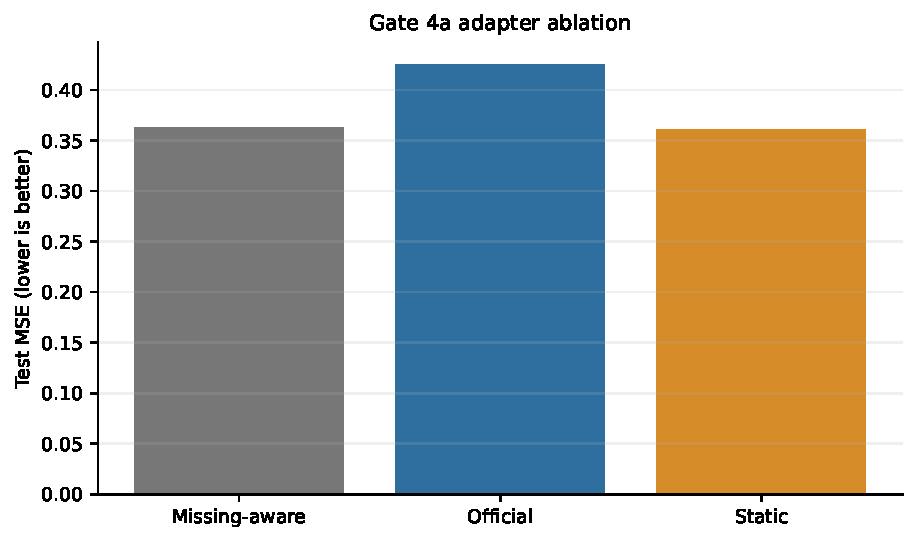
\includegraphics[width=0.78\linewidth]{figA1_gate4a_adapter.pdf}\caption{Adapter MSE comparison.}\label{fig:supp-adapter}\end{figure}

\section{Strict Conformal Negative Result}
\label{supp:conformal}
The additive correction uses a temporally separated calibration set and cannot shrink intervals. It widens the already near-nominal native intervals and does not improve absolute coverage error under this protocol.
\begin{table}[ht]\centering\caption{Formal additive conformal results.}\label{tab:supp-conformal}\scriptsize\begin{tabular}{@{}lrrrrr@{}}
\toprule
Method & Nominal & PICP & MPIW & Coverage error & Interval score \\
\midrule
Mask-severity-conditioned conformal & 0.90 & 0.927136 & 2.262613 & 0.027136 & 2.989775 \\
Marginal conformal & 0.90 & 0.927636 & 2.267989 & 0.027636 & 2.990528 \\
Native & 0.90 & 0.897581 & 1.953189 & 0.002419 & 2.946898 \\
Mask-severity-conditioned conformal & 0.95 & 0.964262 & 2.993500 & 0.014262 & 3.625242 \\
Marginal conformal & 0.95 & 0.964505 & 2.998730 & 0.014505 & 3.625259 \\
Native & 0.95 & 0.937700 & 2.424187 & 0.012300 & 3.596873 \\
\bottomrule
\end{tabular}
\end{table}
\begin{table}[ht]\centering\caption{Conformal mechanism audit; counterfactual rows are diagnostic only.}\label{tab:supp-conformal-mechanism}\scriptsize\resizebox{\linewidth}{!}{\begin{tabular}{@{}lrrrrrr@{}}
\toprule
Head & Nominal & Cal. PICP & Test PICP & Shift & $\hat q$ & $\Delta$ coverage error \\
\midrule
Gaussian & 0.90 & 0.869114 & 0.904533 & 0.035418 & 0.126842 & 0.023728 \\
Gaussian & 0.95 & 0.912017 & 0.937263 & 0.025246 & 0.279881 & 0.001974 \\
Student-t & 0.90 & 0.861667 & 0.897581 & 0.035913 & 0.157400 & 0.025216 \\
Student-t & 0.95 & 0.913178 & 0.937700 & 0.024522 & 0.287271 & 0.002205 \\
\bottomrule
\end{tabular}
}\end{table}
\begin{table}[ht]\centering\caption{All retained probability heads and interval procedures.}\label{tab:supp-conformal-all}\scriptsize\resizebox{\linewidth}{!}{\begin{tabular}{@{}lrrrrrr@{}}
\toprule
Head & Method & Nominal & PICP & MPIW & Coverage error & Interval score \\
\midrule
Gaussian & Mask-severity-conditioned conformal & 0.90 & 0.927797 & 2.289391 & 0.027797 & 2.979145 \\
Gaussian & Marginal conformal & 0.90 & 0.928261 & 2.294196 & 0.028261 & 2.979930 \\
Gaussian & Native & 0.90 & 0.904533 & 2.040512 & 0.004533 & 2.936425 \\
Gaussian & Mask-severity-conditioned conformal & 0.95 & 0.964530 & 2.986506 & 0.014530 & 3.598434 \\
Gaussian & Marginal conformal & 0.95 & 0.964711 & 2.991181 & 0.014711 & 3.598406 \\
Gaussian & Native & 0.95 & 0.937263 & 2.431420 & 0.012737 & 3.571486 \\
Student-t & Mask-severity-conditioned conformal & 0.90 & 0.927136 & 2.262613 & 0.027136 & 2.989775 \\
Student-t & Marginal conformal & 0.90 & 0.927636 & 2.267989 & 0.027636 & 2.990528 \\
Student-t & Native & 0.90 & 0.897581 & 1.953189 & 0.002419 & 2.946898 \\
Student-t & Mask-severity-conditioned conformal & 0.95 & 0.964262 & 2.993500 & 0.014262 & 3.625242 \\
Student-t & Marginal conformal & 0.95 & 0.964505 & 2.998730 & 0.014505 & 3.625259 \\
Student-t & Native & 0.95 & 0.937700 & 2.424187 & 0.012300 & 3.596873 \\
\bottomrule
\end{tabular}
}\end{table}
\begin{figure}[ht]\centering
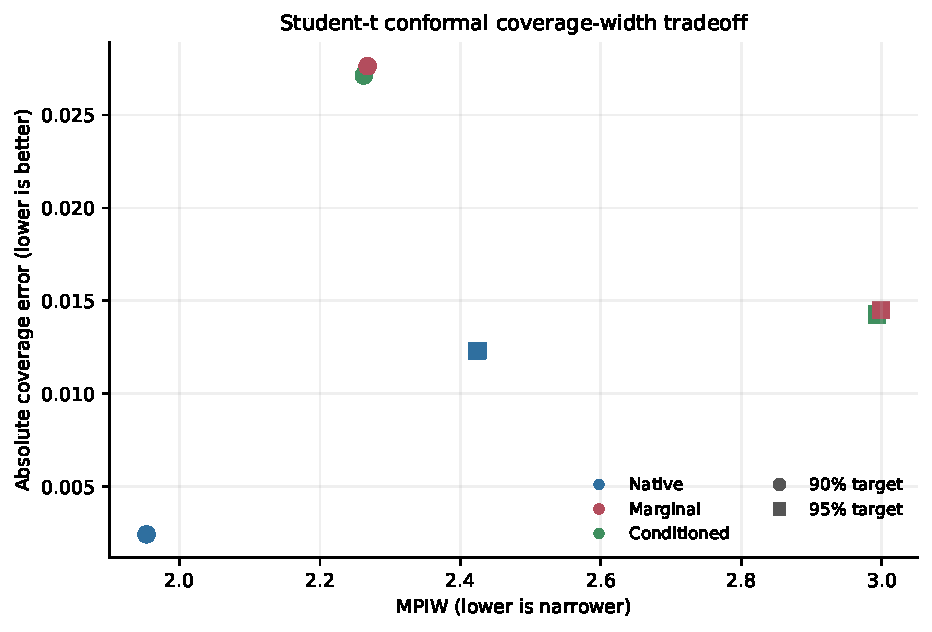
\includegraphics[width=0.48\linewidth]{fig5_conformal_tradeoff.pdf}
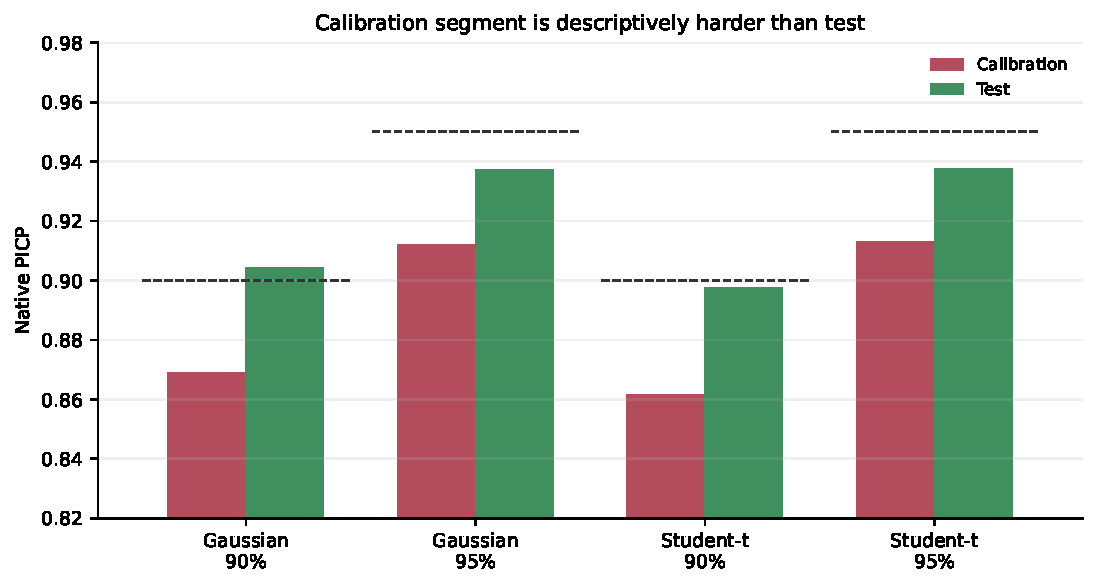
\includegraphics[width=0.48\linewidth]{fig6_calibration_test_shift.pdf}
\caption{Interval-width tradeoff and calibration-to-test coverage shift.}\label{fig:supp-conformal}
\end{figure}
\begin{figure}[ht]\centering
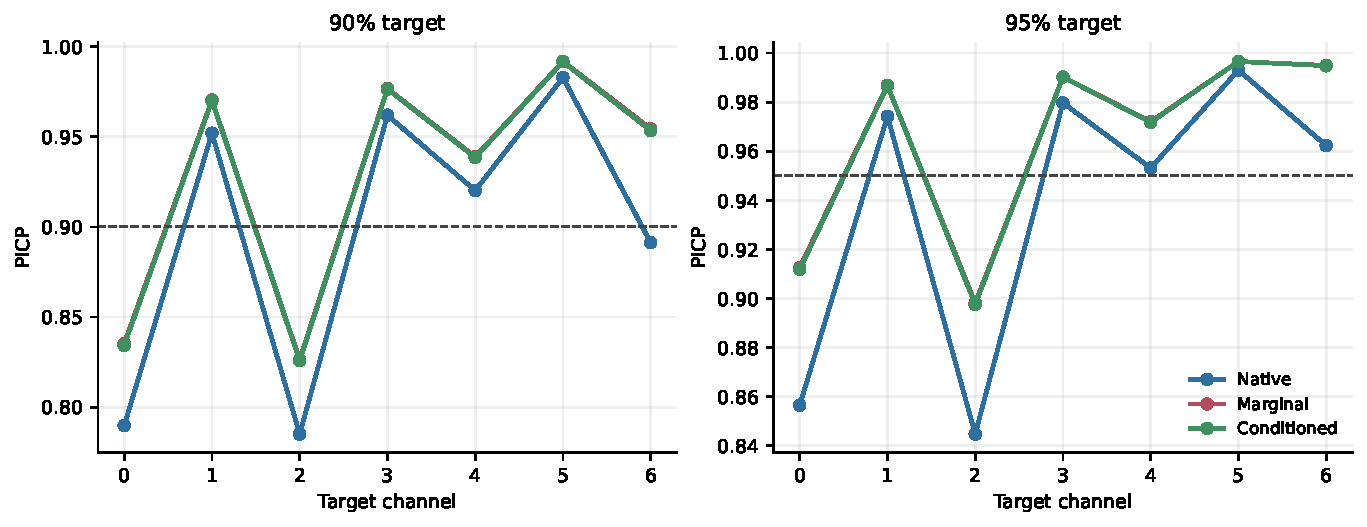
\includegraphics[width=0.48\linewidth]{figA2_gate4c_channel_coverage.pdf}
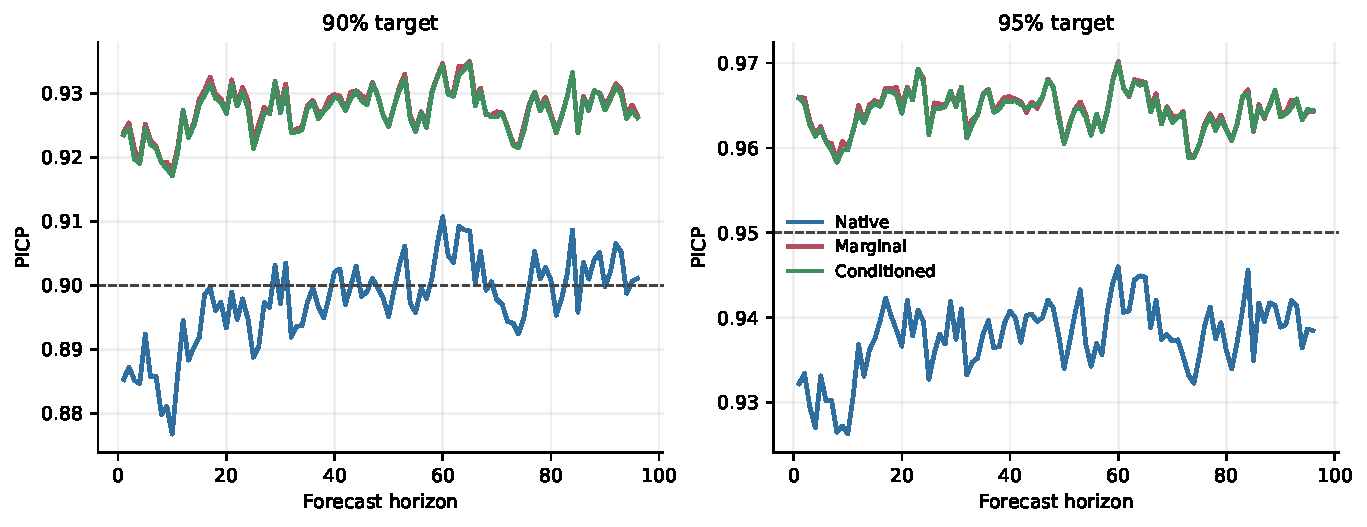
\includegraphics[width=0.48\linewidth]{figA3_gate4c_horizon_coverage.pdf}
\caption{Channel- and horizon-level marginal coverage diagnostics.}\label{fig:supp-coverage}
\end{figure}
